
%(BEGIN_QUESTION)
% Copyright 2013, Tony R. Kuphaldt, released under the Creative Commons Attribution License (v 1.0)
% This means you may do almost anything with this work of mine, so long as you give me proper credit

Identify the type of filtering behavior of the circuit shown in this diagram:

$$\includegraphics[width=15.5cm]{i04774x01.eps}$$

Next, identify the filtering behavior of this same circuit supposing the inductor fails {\it shorted}.  Place two check-marks in the table below to identify each filtering characteristic (one check-mark identifying the healthy circuit's characteristic and another check-mark identifying the faulted circuit's characteristic):

% No blank lines allowed between lines of an \halign structure!
% I use comments (%) instead, so that TeX doesn't choke.

$$\vbox{\offinterlineskip
\halign{\strut
\vrule \quad\hfil # \ \hfil & 
\vrule \quad\hfil # \ \hfil & 
\vrule \quad\hfil # \ \hfil \vrule \cr
\noalign{\hrule}
%
% First row
{\bf Filter type} & {\bf Healthy circuit} & {\bf Faulted circuit} \cr
%
\noalign{\hrule}
%
% Another row
Low-pass &  &  \cr
%
\noalign{\hrule}
%
% Another row
High-pass &  &  \cr
%
\noalign{\hrule}
%
% Another row
Band-pass &  &  \cr
%
\noalign{\hrule}
%
% Another row
Band-stop &  &  \cr
%
\noalign{\hrule}
%
% Another row
Passes all frequencies &  &  \cr
%
\noalign{\hrule}
%
% Another row
Blocks all frequencies &  &  \cr
%
\noalign{\hrule}
} % End of \halign 
}$$ % End of \vbox

\underbar{file i04774}
%(END_QUESTION)





%(BEGIN_ANSWER)

% No blank lines allowed between lines of an \halign structure!
% I use comments (%) instead, so that TeX doesn't choke.

$$\vbox{\offinterlineskip
\halign{\strut
\vrule \quad\hfil # \ \hfil & 
\vrule \quad\hfil # \ \hfil & 
\vrule \quad\hfil # \ \hfil \vrule \cr
\noalign{\hrule}
%
% First row
{\bf Filter type} & {\bf Healthy circuit} & {\bf Faulted circuit} \cr
%
\noalign{\hrule}
%
% Another row
Low-pass &  & $\surd$ \cr
%
\noalign{\hrule}
%
% Another row
High-pass &  &  \cr
%
\noalign{\hrule}
%
% Another row
Band-pass &  &  \cr
%
\noalign{\hrule}
%
% Another row
Band-stop & $\surd$ &  \cr
%
\noalign{\hrule}
%
% Another row
Passes all frequencies &  &  \cr
%
\noalign{\hrule}
%
% Another row
Blocks all frequencies &  &  \cr
%
\noalign{\hrule}
} % End of \halign 
}$$ % End of \vbox


%(END_ANSWER)





%(BEGIN_NOTES)

{\bf This question is intended for exams only and not worksheets!}.

%(END_NOTES)


